%% This is file `elsarticle-template-2-harv.tex',
%%
%% Copyright 2009 Elsevier Ltd
%%
%% This file is part of the 'Elsarticle Bundle'.
%% ---------------------------------------------
%%
%% It may be distributed under the conditions of the LaTeX Project Public
%% License, either version 1.2 of this license or (at your option) any
%% later version.  The latest version of this license is in
%%    http://www.latex-project.org/lppl.txt
%% and version 1.2 or later is part of all distributions of LaTeX
%% version 1999/12/01 or later.
%%
%% The list of all files belonging to the 'Elsarticle Bundle' is
%% given in the file `manifest.txt'.
%%
%% Template article for Elsevier's document class `elsarticle'
%% with harvard style bibliographic references
%%
%% $Id: elsarticle-template-2-harv.tex 155 2009-10-08 05:35:05Z rishi $
%% $URL: http://lenova.river-valley.com/svn/elsbst/trunk/elsarticle-template-2-harv.tex $
%%

%%\documentclass[preprint,authoryear,12pt]{elsarticle}

%% Use the option review to obtain double line spacing
%% \documentclass[authoryear,preprint,review,12pt]{elsarticle}

%% Use the options 1p,twocolumn; 3p; 3p,twocolumn; 5p; or 5p,twocolumn
%% for a journal layout:

%% Astronomy & Computing uses 5p
%% \documentclass[final,authoryear,5p,times]{elsarticle}
\documentclass[final,authoryear,5p,times,twocolumn]{elsarticle}

%% if you use PostScript figures in your article
%% use the graphics package for simple commands
%% \usepackage{graphics}
%% or use the graphicx package for more complicated commands
\usepackage{graphicx}
%% or use the epsfig package if you prefer to use the old commands
%% \usepackage{epsfig}

%% The amssymb package provides various useful mathematical symbols
\usepackage{amssymb}
%% The amsthm package provides extended theorem environments
%% \usepackage{amsthm}

\usepackage[pdftex,pdfpagemode={UseOutlines},bookmarks,bookmarksopen,colorlinks,linkcolor={blue},citecolor={green},urlcolor={red}]{hyperref}
\usepackage{hypernat}

%% The lineno packages adds line numbers. Start line numbering with
%% \begin{linenumbers}, end it with \end{linenumbers}. Or switch it on
%% for the whole article with \linenumbers after \end{frontmatter}.
%% \usepackage{lineno}

%% natbib.sty is loaded by default. However, natbib options can be
%% provided with \biboptions{...} command. Following options are
%% valid:

%%   round  -  round parentheses are used (default)
%%   square -  square brackets are used   [option]
%%   curly  -  curly braces are used      {option}
%%   angle  -  angle brackets are used    <option>
%%   semicolon  -  multiple citations separated by semi-colon (default)
%%   colon  - same as semicolon, an earlier confusion
%%   comma  -  separated by comma
%%   authoryear - selects author-year citations (default)
%%   numbers-  selects numerical citations
%%   super  -  numerical citations as superscripts
%%   sort   -  sorts multiple citations according to order in ref. list
%%   sort&compress   -  like sort, but also compresses numerical citations
%%   compress - compresses without sorting
%%   longnamesfirst  -  makes first citation full author list
%%
%% \biboptions{longnamesfirst,comma}

% \biboptions{}

\journal{Astronomy \& Computing}

%% Make single quotes look right in verbatim mode
\usepackage{upquote}

\begin{document}

\begin{frontmatter}

%% Title, authors and addresses

%% use the tnoteref command within \title for footnotes;
%% use the tnotetext command for the associated footnote;
%% use the fnref command within \author or \address for footnotes;
%% use the fntext command for the associated footnote;
%% use the corref command within \author for corresponding author footnotes;
%% use the cortext command for the associated footnote;
%% use the ead command for the email address,
%% and the form \ead[url] for the home page:
%%
%% \title{Title\tnoteref{label1}}
%% \tnotetext[label1]{}
%% \author{Name\corref{cor1}\fnref{label2}}
%% \ead{email address}
%% \ead[url]{home page}
%% \fntext[label2]{}
%% \cortext[cor1]{}
%% \address{Address\fnref{label3}}
%% \fntext[label3]{}

\title{FellWalker - a Clump Identification Algorithm }

%% use optional labels to link authors explicitly to addresses:
%% \author[label1,label2]{<author name>}
%% \address[label1]{<address>}
%% \address[label2]{<address>}

\author[jac]{David S.\ Berry\corref{cor1}}
\ead{d.berry@jach.hawaii.edu}

\cortext[cor1]{Corresponding author}

\address[jac]{Joint Astronomy Centre, 660 N.\ A`oh\=ok\=u Place, Hilo, HI
  96720, USA}

\begin{abstract}
%% Text of abstract

This paper describes the FellWalker algorithm, which segments a 1-, 2- or
3-dimensional array of data values into a set of disjoint clumps of
emission, each containing a single significant peak. Pixels below a
nominated constant data level are assumed to be background pixels and are
not assigned to any clump. FellWalker is thus equivalent in purpose to
the CLUMPFIND algorithm. However, unlike CLUMPFIND, which segments the
array on the basis of a set of evenly-spaced contours and thus uses only
a small fraction of the available data  values, the FellWalker algorithm
is based on a gradient-tracing scheme which uses all available data values.

\end{abstract}

\begin{keyword}
%% keywords here, in the form: keyword \sep keyword

%% MSC codes here, in the form: \MSC code \sep code
%% or \MSC[2008] code \sep code (2000 is the default)

clump identification \sep
Starlink

\end{keyword}

\end{frontmatter}

% \linenumbers

%% Journal abbreviations
\newcommand{\mnras}{Mon Not R Astron Soc}
\newcommand{\aap}{Astron Astrophys}
\newcommand{\aaps}{Astron Astrophys Supp}
\newcommand{\pasp}{Pub Astron Soc Pacific}
\newcommand{\apj}{Astrophys J}
\newcommand{\apjs}{Astrophys J Supp}
\newcommand{\qjras}{Quart J R Astron Soc}
\newcommand{\an}{Astron.\ Nach.}
\newcommand{\ijimw}{Int.\ J.\ Infrared \& Millimeter Waves}
\newcommand{\procspie}{Proc.\ SPIE}
\newcommand{\aspconf}{ASP Conf. Ser.}

%% ASCL
\newcommand{\ascl}[1]{\href{http://www.ascl.net/#1}{ascl:#1}}

%% main text
\section{Introduction}
\label{sec:intro}

The CLUMPFIND algorithm \citep[][\ascl{1107.014}]{1994Williams} has been widely used for
decomposing 2- and 3-dimensional data into disjoint clumps of emission,
each associated with a single significant peak. It is based upon an
analysis of a set of evenly spaced contours derived from the data array
and has two main parameters - the lowest contour level, below which
data is ignored, and the interval between contours. However it has been
noted by \cite{2009Pineda} that the decomposition produced by CLUMPFIND
can be very sensitive to the specific value used for the contour interval,
particularly for 3-dimensional data and crowded fields. The choice of an
optimal contour interval is a compromise - real peaks may be missed if
the interval is too large, but noise spikes may be interpreted as real
peaks if the interval is too small.

The FellWalker algorithm attempts to circumvent these issues by avoiding
the use of contours altogether. Only a small fraction of the available
pixel values fall on the contour levels used by CLUMPFIND - the majority
fall \emph{between} these levels and so will have no effect on the
resulting decomposition. By contrast, FellWalker makes equal use of all
available pixel values above a stated threshold.

The name ``Fell Walker'' relates to the popular British pass-time of
walking up the hills and mountains of northern England, particularly
those of the Lake District
(\htmladdnormallink{http://en.wikipedia.org/wiki/Hillwalking}~), and was
chosen to reflect the way in which the algorithm proceeds iteratively by
following an upward path from a low-valued pixel to a significant summit
or peak in data-value. The following description of the algorithm uses
this fell-walking metaphor at frequent intervals.

\begin{figure}
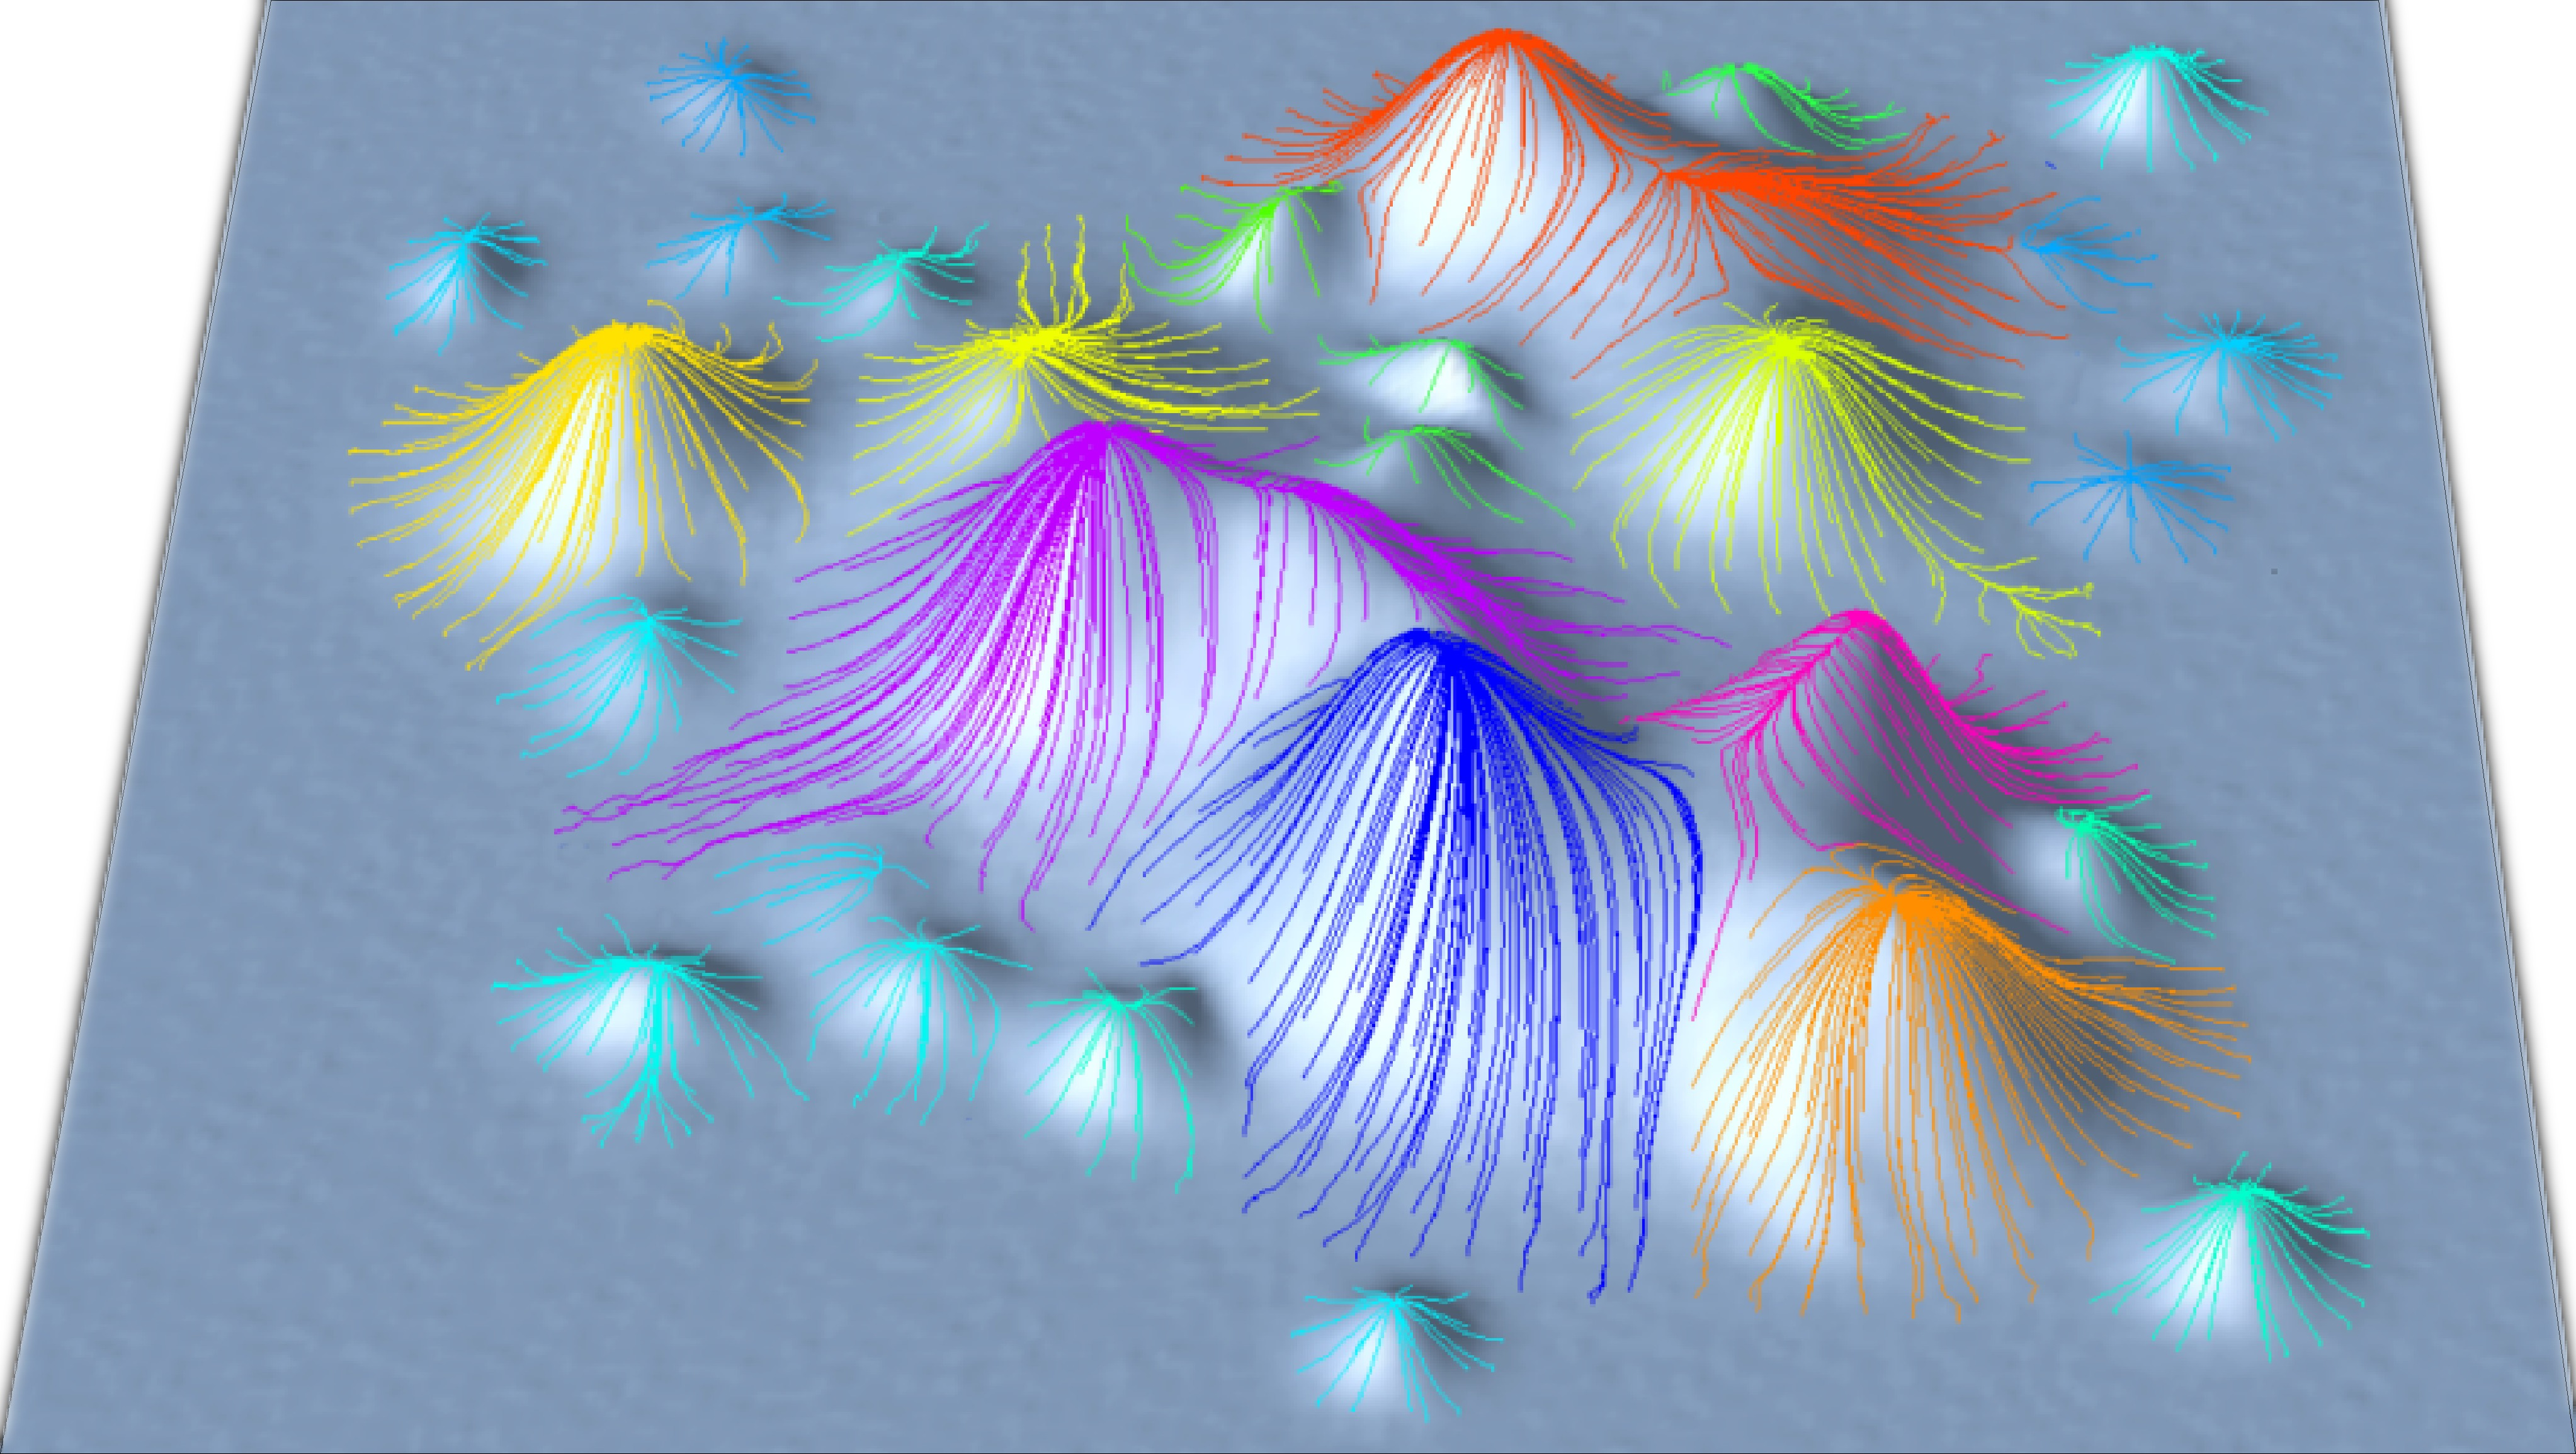
\includegraphics[width=\columnwidth]{fellwalking}
\caption{In 2-dimensions, peaks in data value are reminiscent of the
fells of northern England. The FellWalker algorithm performs many walks
starting at various low-land pixels, and for each one follows a line of steepest ascent
until a significant summit is reached. All walks that terminate at the
same peak are assigned to the same clump.}
\label{fig:fellwalking}
\end{figure}

\section{The FellWalker Algorithm}

The core of the FellWalker algorithm consists of repeatedly following
different paths of steepest ascent in order to reach a significant
summit, each of which is associated with a clump, as illustrated in
Fig.~\ref{fig:fellwalking}. Every pixel with a data value above a
user-specified threshold is used in turn as the start of a ``walk''. A
walk consists of a series of steps, each of which takes the algorithm
from the current pixel to an immediately neighbouring pixel of higher
value, until a pixel is found which is higher than any of its neighbours.
When this happens, a search for a higher pixel is made over a larger
neighbourhood. If such a pixel is found the walk continues from this
higher pixel. If no higher pixel is found it is assumed that a new summit
has been reached - a new clump identifier is issued and all pixels
visited on the walk are assigned to the new clump. If at any point a walk
encounters a pixel which has already been assigned to a clump, then all
pixels so far visited on the walk are assigned to that same clump and the
walk terminates.

It is possible for this basic algorithm to fragment up-land plateau
regions into lots of small clumps which are well separated spatially but
have minimal dips between them. The raw clumps identified by the above
process can be merged to avoid such fragmentation, on the basis of a
user-specified minimum dip between clumps. These merged clumps may,
optionally, be cleaned by smoothing their boundaries using a single step
of a cellular automaton.

Finally, each clump is characterised using a number of statistics, and a
catalogue of clumps statistics is created together with a pixel mask
identifying the clump to which each pixel is assigned.

The following sections give more detailed descriptions of each of these
phases in the FellWalker algorithm.

\subsection{Identifying Raw Clumps}
An array of integer values is first allocated, which is the same shape
and size as the supplied data array. This ``clump assignment array''
(CAA) is used to record the integer identifier of the clump, if any, to
which each pixel has been assigned. All clump identifiers are greater
than zero. An initial pass is made through the supplied data array to
identify pixels which have data values above a user-specified threshold
value. Such pixels are assigned a value of zero in the CAA indicating
that the pixel is usable but has not yet been assigned to a clump, and
all other pixels are assigned a value of -1 indicating that the pixel is
unusable and should never be assigned to a clump.

This initial CAA is then searched for any isolated individual pixels
above the threshold. Such pixels are set to -1 in the CAA, indicating
they should be ignored.

The main loop is then entered, which considers each pixel in turn as the
potential start of a walk to a peak. Pixels which have a non-zero value
in the CAA are skipped since they have either already been assigned to a
clump (if the CAA value is positive) or have been flagged as unusable (if
the CAA value is negative). A single walk consists of stepping from pixel
to pixel until a pixel is reached which is already known to be part of a
clump, or significant isolated peak is encountered. The vector indicies of
the pixels visited along a walk are recorded in a temporary array so that
they  can be identified later.

At each step, the pixel values within a box of width three pixels are compared
to the central pixel to find the neighbouring pixel which give the highest
gradient\footnote{This gradient takes into account the fact that corner
pixels are further away from the box centre than mid-side pixels.}. Thus
2 neighbours are checked if the data is 1-dimensional data, 8 are
checked if the data is 2-dimensional and 26 are checked if the data is
3-dimensional.

If the highest gradient found above is greater than zero - that is, if
there is an upward route out of the current pixel - the walk steps to the
selected neighbouring pixel. If this new pixel has already been assigned
to a clump (\emph{i.e.} if the CAA holds a positive value at the new
pixel), then the new walk has joined an older walk and so will eventually
end up at the same peak as the older walk. The existing positive CAA
value of the new pixel (\emph{i.e.} the clump index assigned to the older
walk) is copied into the CAA for all pixels visited so far on the new
walk, and a new walk from the next starting pixel is initiated.

If the highest gradient found to any neighbouring pixel is less than or
equal to zero, then there is no upward route from the central pixel. This
could mean the walk has reached a significant peak, but it could also
mean it has merely reached a noise spike. To distinguish these two cases,
a search is made over a larger box\footnote{By default a box of width 9
pixels, but the user can specify a different size.}. If the maximum pixel
value in this larger box is smaller than the central pixel value, then
the central pixel is considered to be a significant peak. A new clump
identifier is issued for it and stored in the CAA at all pixels visited
on the walk. A new walk from the next starting pixel is then initiated.

If the maximum pixel value found in the larger box is greater than the
central pixel value, then the central pixel is considered to be a noise
spike. The walk then ``jumps across the gap'' and continues from the
highest pixel found in the box.

\begin{figure}
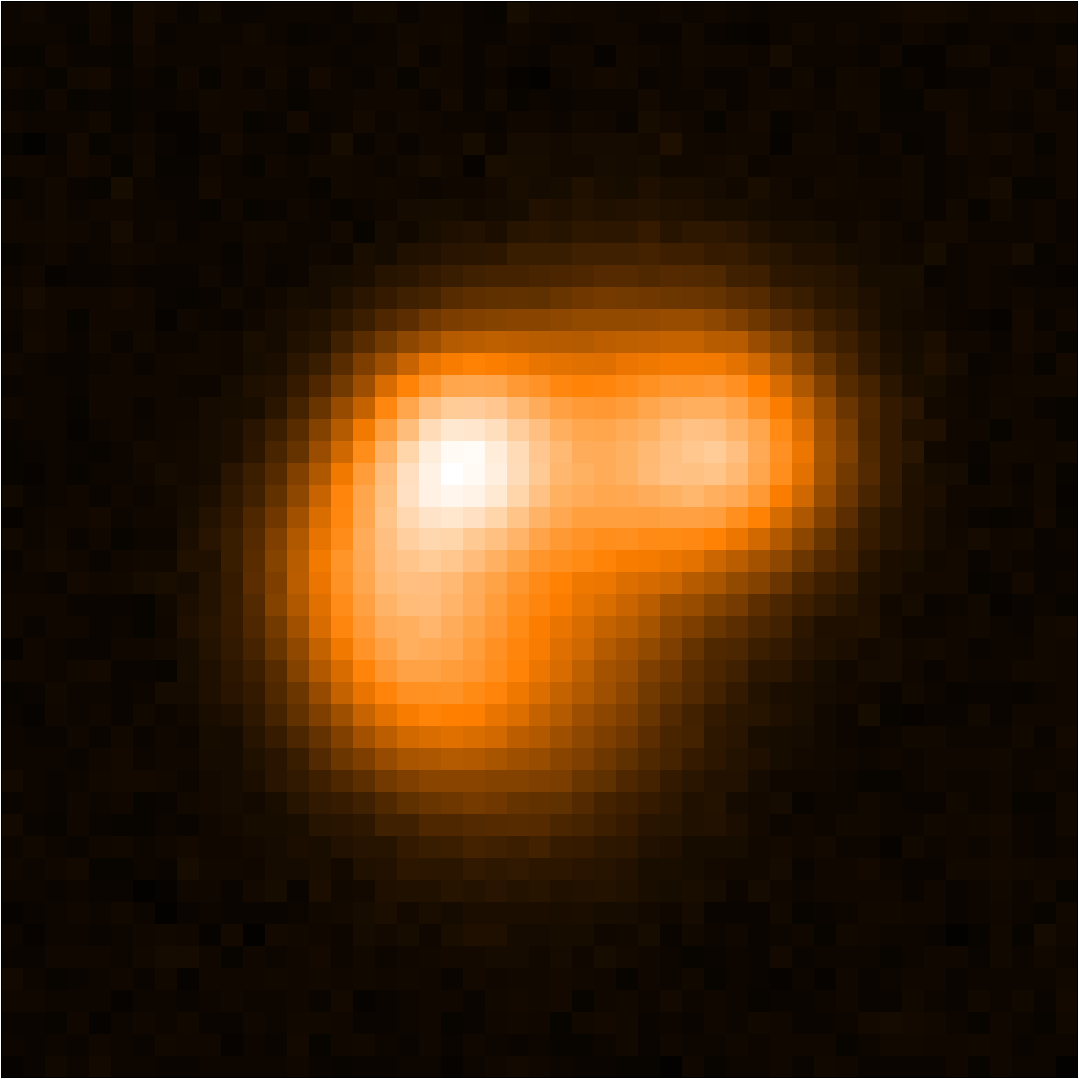
\includegraphics[width=\columnwidth]{sim}
\caption{A 50x50 array of artificial data used to illustrate the
FellWalker algorithm below.}
\label{fig:sim}
\end{figure}

\begin{figure}
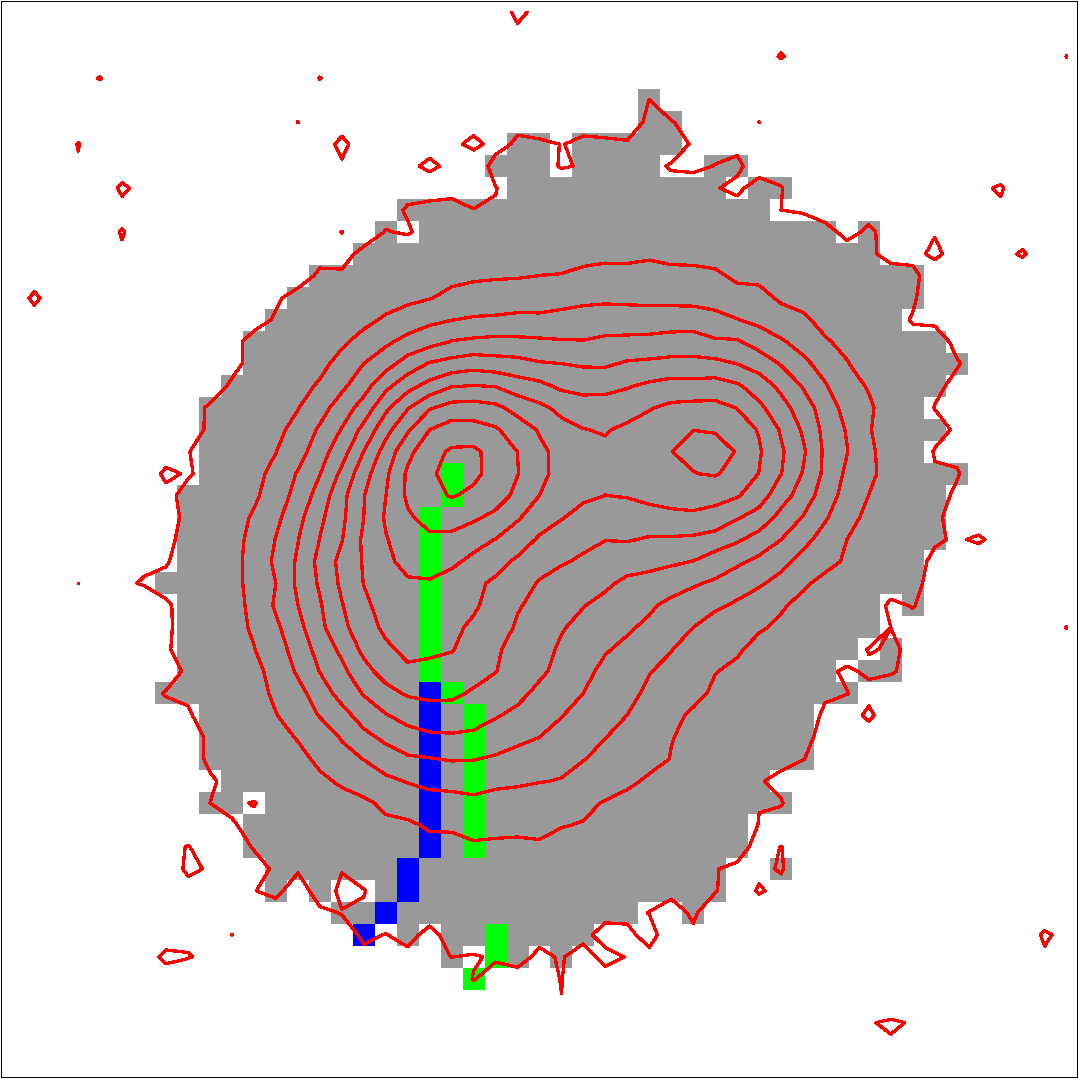
\includegraphics[width=\columnwidth]{walks}
\caption{Two walks up a peak within the artificial data shown in
Fig.~\ref{fig:sim}. The contours show the data values themselves. The white
background pixels are below the nominated threshold, the grey pixels are
above the threshold but have not yet been assigned to a clump. The green
pixels trace the first walk that reached the left-hand peak. The blue pixels
trace a later walk to the same peak that was terminated when it met the first
walk. The green and blue pixels are all assigned to the same clump. These
walks follow the steepest line of ascent. Note the gap in the green line
near its start at the lowest contour - this is where a jump was made from
a noise spike to the highest value in a 9x9 box of neighbouring pixels.}

\label{fig:walks}
\end{figure}

The above process results in the CAA holding a clump identifier for every
usable pixel in the supplied data array. However, some of the walks
performed above may start with a section of very low gradient before any
significant ascent begins. The user is allowed to specify a minimum
gradient which must be achieved before a walk is considered to have
begun. Any section of the walk that occurs before the first such
``steep'' section is flagged as unusable in the CAA. For this test,
the gradient of a walk is averaged over four consecutive steps.

This process is illustrated in Fig.~\ref{fig:walks} which shows two
example up-hill walks produced by FellWalker for the artificial data shown
in Fig.~\ref{fig:sim}. The final CAA produced by the above process for
this data is shown in Fig.~\ref{fig:rawmask}.

\begin{figure}
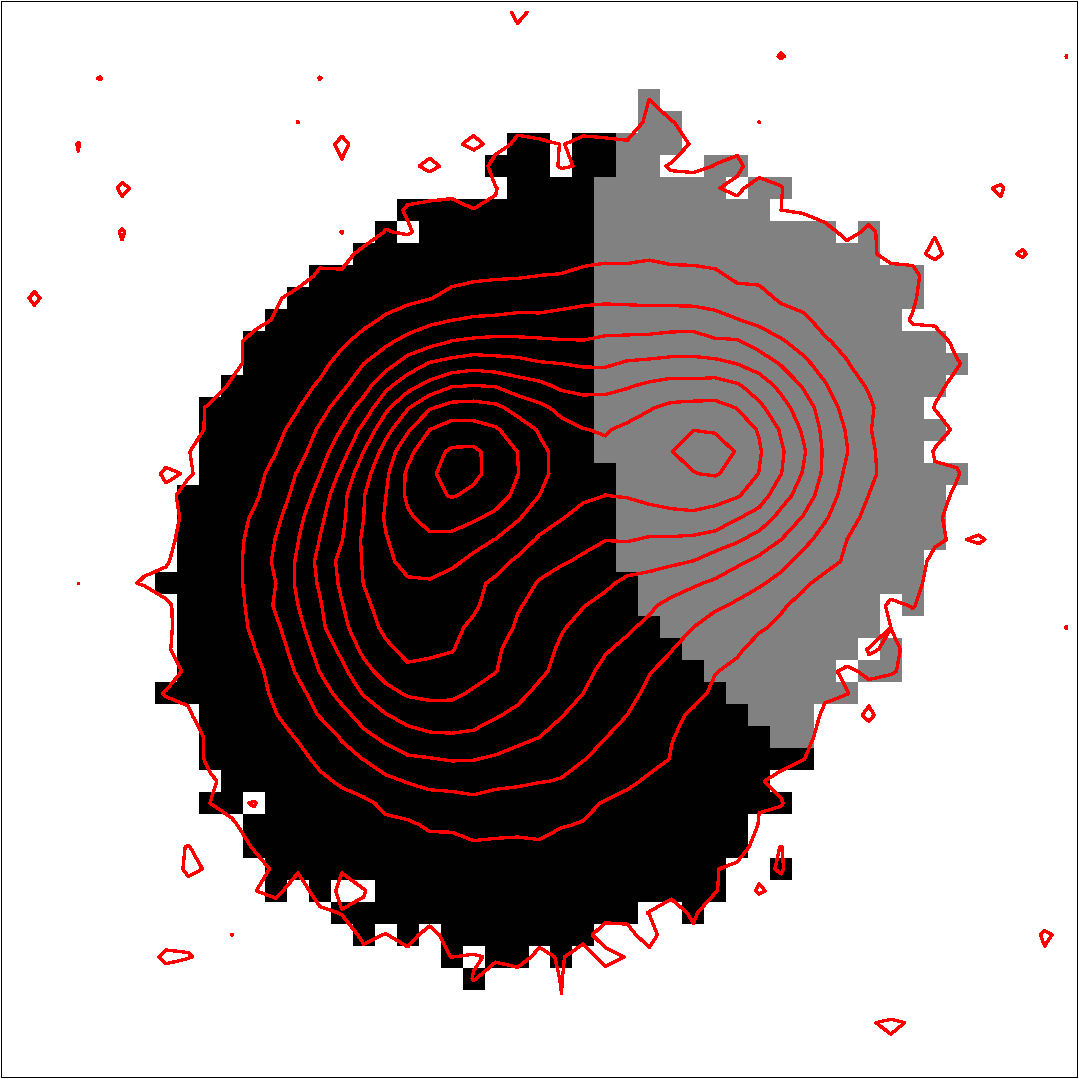
\includegraphics[width=\columnwidth]{rawmask}
\caption{The raw clump mask created for the artificial data shown in
Fig.~\ref{fig:sim}. Two clumps are found, indicated by the black and grey
pixels.}
\label{fig:rawmask}
\end{figure}


\subsection{Merging Clumps}

The number of significant peaks found by the above process is determined
primarily by the maximum distance a walk can jump when searching for a
higher neighbouring pixel value. This parameter - known as \emph{MaxJump}
- defaults to 4 pixels. Using a larger value results in more local peaks
being interpreted as noise spikes rather than significant peaks, with a
corresponding reduction in the number of significant peaks found. Thus at
this point, peaks are discriminated simply on the basis of their spatial
separation.

This means it is possible for a clump with a wide, flat summit to be
fragmented into multiple clumps on the basis of noise spikes that are
separated by more than \emph{MaxJump} pixels.

To correct this, FellWalker merges adjacent clumps if the ``valley''
between the two adjacent peaks is very shallow.

Each clump (referred to as the ``central'' clump below) is considered in
turn to see if it should be merged with any of its neighbouring clumps.
The height of the ``col\footnote{The highest point on the boundary
between the two clumps.}'' between the central clump and each
neighbouring clump is found in turn, and the neighbouring clump with the
highest col is selected as a candidate for merging. If the peak value in
the central clump is less than a specified value,
\emph{MinDip}\footnote{The default is three times the noise level in the
data.}, above the col, the two clumps are merged into a single clump.

Once all central clumps have been checked in this way, the whole process
is repeated to see if any of the merged clumps should themselves be
merged. This process repeats until no further clumps can be merged.

\subsection{Cleaning Clump Outlines}

Once neighbouring clumps separated by shallow valleys have been merged,
there is an option to smooth the boundaries between adjacent clumps to
reduce the effects of noise. This is done using a specified number of
steps of a cellular automaton to modify the integer values in the CAA.

A single step creates a new CAA from the old CAA. Each pixel in the new
CAA is set to the most commonly occurring clump index within a box of
width 3 pixels centred on the corresponding pixel within the old CAA. The
output CAA from one step becomes the input CAA to the next step. By
default, only one step is performed. Fig.~\ref{fig:cleanedmask} shows the
effects of applying a single step to the CAA shown in Fig.~\ref{fig:rawmask}.

\begin{figure}
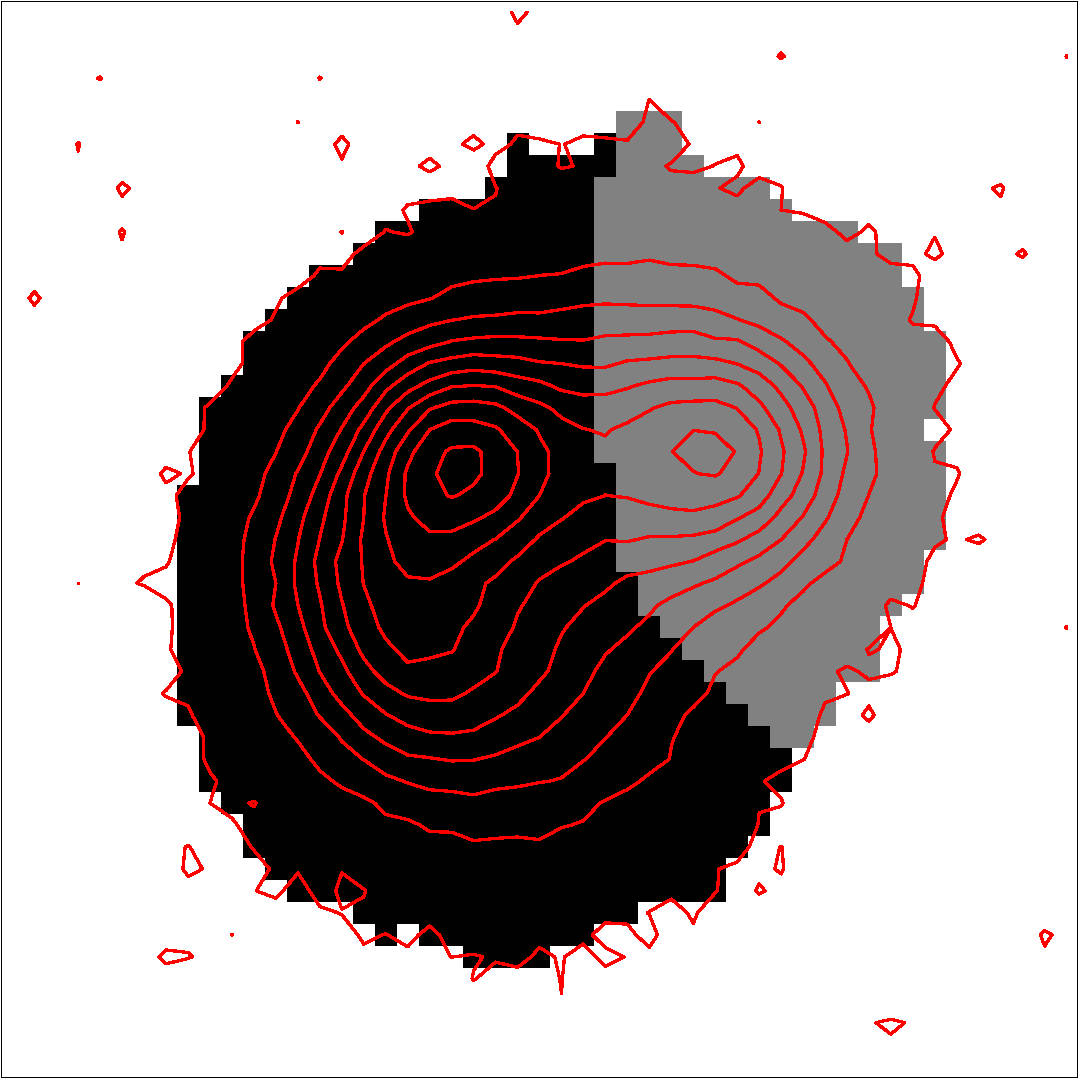
\includegraphics[width=\columnwidth]{cleaned}
\caption{The smoothing effect of a single step of the cellular automaton
on the clump outlines shown in Fig.~\ref{fig:rawmask}.}
\label{fig:cleanedmask}
\end{figure}


\subsection{Characterising Each Clump}
The FellWalker algorithm is implemented within the {\tt findclumps}
command of the Starlink CUPID package (see section~\ref{sec:cupid}). This
command implements several other clump finding algorithms, and one of its
design requirements was that each algorithm should characterise clumps in
the same way, so that results from different algorithms can be compared
directly. Thre results are presented in the following ways:

\begin{enumerate}

\item A pixel mask which is the same shape and size as the supplied data
array. Each pixel value is an integer which gives the index of the clump
to which the pixel has been assigned. Pixels that have not been assigned
to any clump are flagged with a special value.

\item A set of minimal cut-outs from the supplied data array. Each cut-out
holds the supplied pixels values corresponding to a single clump, with pixels
outside the clump set to a special ``blank'' value.

\item A table in which each row describes a single clump. The columns are:

\begin{description}
\item[Peak1] The position of the clump peak value on axis 1.
\item[Peak2] The position of the clump peak value on axis 2.
\item[Peak3] The position of the clump peak value on axis 3.
\item[Cen1] The position of the clump centroid on axis 1.
\item[Cen2] The position of the clump centroid on axis 2.
\item[Cen3] The position of the clump centroid on axis 3.
\item[Size1] The size of the clump along pixel axis 1.
\item[Size2] The size of the clump along pixel axis 2.
\item[Size3] The size of the clump along pixel axis 3.
\item[Sum] The total data sum in the clump.
\item[Peak] The peak value in the clump.
\item[Volume] The total number of pixels falling within the clump.
\end{description}

There is also an optional column called ``Shape'' containing an STC-S
description \citep{2007STCS,2010ASPC..434..213B} of
the spatial coverage of each clump.

\end{enumerate}



\section{\label{sec:cupid}CUPID - an Implementation of FellWalker}
The Starlink CUPID package \citep[][\ascl{1311.007}]{CupidAdass,SUN255} provides
implementations of various clump-finding algorithms, including FellWalker
and CLUMPFIND. In common with the rest of the Starlink software \citep[][\ascl{1110.012}]{StarlinkAdass},
the source code for the CUPID package is open-source and is available on github at
\htmladdnormallink{https://github.com/Starlink}.

\section{Comparing FellWalker and CLUMPFIND}

Include some references to earlier investigations? \citep[e.g.][]{2010Watson}

May want to consider \citep{2012PASA...29..301W} which uses
DUCHAMP \citep[][\ascl{1201.011}]{2012MNRAS.421.3242W}.

\subsection{Simulated Data}

\subsection{Real Sub-millimetre Data}


\section{Acknowledgements}

The Starlink software is currently maintained by the Joint Astronomy
Centre, Hawaii with support from the UK Science and Technology
Facilities Council.


%% The Appendices part is started with the command \appendix;
%% appendix sections are then done as normal sections
%% \appendix

%% \section{}
%% \label{}

%% References
%%
%% Following citation commands can be used in the body text:
%%
%%  \citet{key}  ==>>  Jones et al. (1990)
%%  \citep{key}  ==>>  (Jones et al., 1990)
%%
%% Multiple citations as normal:
%% \citep{key1,key2}         ==>> (Jones et al., 1990; Smith, 1989)
%%                            or  (Jones et al., 1990, 1991)
%%                            or  (Jones et al., 1990a,b)
%% \cite{key} is the equivalent of \citet{key} in author-year mode
%%
%% Full author lists may be forced with \citet* or \citep*, e.g.
%%   \citep*{key}            ==>> (Jones, Baker, and Williams, 1990)
%%
%% Optional notes as:
%%   \citep[chap. 2]{key}    ==>> (Jones et al., 1990, chap. 2)
%%   \citep[e.g.,][]{key}    ==>> (e.g., Jones et al., 1990)
%%   \citep[see][pg. 34]{key}==>> (see Jones et al., 1990, pg. 34)
%%  (Note: in standard LaTeX, only one note is allowed, after the ref.
%%   Here, one note is like the standard, two make pre- and post-notes.)
%%
%%   \citealt{key}          ==>> Jones et al. 1990
%%   \citealt*{key}         ==>> Jones, Baker, and Williams 1990
%%   \citealp{key}          ==>> Jones et al., 1990
%%   \citealp*{key}         ==>> Jones, Baker, and Williams, 1990
%%
%% Additional citation possibilities
%%   \citeauthor{key}       ==>> Jones et al.
%%   \citeauthor*{key}      ==>> Jones, Baker, and Williams
%%   \citeyear{key}         ==>> 1990
%%   \citeyearpar{key}      ==>> (1990)
%%   \citetext{priv. comm.} ==>> (priv. comm.)
%%   \citenum{key}          ==>> 11 [non-superscripted]
%% Note: full author lists depends on whether the bib style supports them;
%%       if not, the abbreviated list is printed even when full requested.
%%
%% For names like della Robbia at the start of a sentence, use
%%   \Citet{dRob98}         ==>> Della Robbia (1998)
%%   \Citep{dRob98}         ==>> (Della Robbia, 1998)
%%   \Citeauthor{dRob98}    ==>> Della Robbia


%% References with bibTeX database:

\bibliographystyle{model2-names-astronomy}
\bibliography{fellwalker}

%% Authors are advised to submit their bibtex database files. They are
%% requested to list a bibtex style file in the manuscript if they do
%% not want to use model2-names.bst.

%% References without bibTeX database:

% \begin{thebibliography}{00}

%% \bibitem must have one of the following forms:
%%   \bibitem[Jones et al.(1990)]{key}...
%%   \bibitem[Jones et al.(1990)Jones, Baker, and Williams]{key}...
%%   \bibitem[Jones et al., 1990]{key}...
%%   \bibitem[\protect\citeauthoryear{Jones, Baker, and Williams}{Jones
%%       et al.}{1990}]{key}...
%%   \bibitem[\protect\citeauthoryear{Jones et al.}{1990}]{key}...
%%   \bibitem[\protect\astroncite{Jones et al.}{1990}]{key}...
%%   \bibitem[\protect\citename{Jones et al., }1990]{key}...
%%   \harvarditem[Jones et al.]{Jones, Baker, and Williams}{1990}{key}...
%%

% \bibitem[ ()]{}

% \end{thebibliography}

\end{document}

%%
%% End of file `elsarticle-template-2-harv.tex'.
